In the rapidly evolving landscape of India's social and romantic interactions, the surge in online dating platforms like Bumble has marked a significant shift in how relationships are formed and nurtured. This shift, driven by technological advancements and changing cultural attitudes, underscores the critical importance of studying anti-discrimination within these digital realms. As internet usage in India reached an unprecedented 1.3 billion by 2023 \cite{statista_internet_users_2050}, the role of algorithms in shaping social dynamics becomes increasingly pertinent. Our research delves into the complexities of algorithmic bias and discrimination on Bumble, an online dating platform that has gained popularity among Indian users. By integrating insights from AI fairness and inclusion studies, we aim to dissect the algorithmic underpinnings that could perpetuate discrimination in the digital dating scene.

Online dating applications, which involve creating user profiles to search for and communicate with potential partners, have become a cornerstone of modern romantic and social interactions. These platforms employ various technologies, including location-based services and sophisticated algorithms, to suggest compatible partners to users. Specifically, Bumble's recommendation algorithm, which is speculated to utilize an "Elo Score" similar to that of Tinder, plays a pivotal role in this process. This score, a measure of desirability rather than mere attractiveness, is determined by a user's interaction patterns, such as "swipes" on profiles, as well as how other users interact with their profile. Despite the opacity surrounding the exact mechanics of these recommendation engines, it is evident that their effectiveness hinges on the representativeness and quality of the training data used.

However, the deployment of such algorithms raises concerns regarding the potential reinforcement of mainstream content while sidelining diverse and minority perspectives.\cite{davidson-etal-2019-racial} This issue, likely stemming from inadequate representation within the data, leads to a skewed presentation of profiles that disproportionately reflects prevailing societal preferences. The consequent narrowing of content diversity not only reinforces pre-existing cultural biases but also limits the exposure range to a homogeneous set of ideas and individuals. Our investigation into Bumble's algorithm seeks to critically evaluate how these dynamics affect interpersonal interactions and self-presentation on the platform.

Furthermore, our study places a particular emphasis on examining the discrepancies and biases in the recommendations made to individuals of dominant genders, such as men and women, compared to those identifying with non-binary genders. This exploration is crucial for uncovering any inherent algorithmic biases and discussing their broader implications for digital social interactions and inclusivity. By doing so, we aim to illuminate the ways in which digital technologies, through their algorithmic decisions, wield power and influence over social life. As this research progresses, it leads us to ponder deeper questions regarding the intersection of technology, society, and the fabric of our interpersonal relationships. Through this comprehensive analysis, we contribute to the ongoing dialogue on AI fairness and strive to foster a more inclusive digital environment where technology serves as a bridge rather than a barrier to social connectivity and understanding.

%----------------------------------------------
\section{Evolution of Dating and Matrimony Technologies}

\subsection{The West}
The history of dating and matrimony in Western societies has evolved significantly over the centuries, shaped by social, economic, religious, and technological changes. This evolution reflects broader shifts in attitudes toward marriage, gender roles, and social interactions. Pre-19th Century, marriages were arranged for political or economic alliances, and love was not considered as a prerequisite for marriage.  It was in the late 18th century that emotions and love started to play a role in matrimony. Newspapers played a crucial role in this evolution. Initially, matrimonial advertisements in newspapers were straightforward, focusing on the financial and social status of individuals seeking spouses. These ads were practical, aiming to match families for mutual economic benefit rather than love. However, as romantic love became more central to marriage, the nature of these advertisements began to change.

By the late 19th and early 20th centuries, personal ads in newspapers started reflecting the shift towards companionate marriage. These ads became more personal and emotional, with individuals describing their personal qualities, interests, and desires for a compatible partner rather than focusing solely on financial stability or social status. This change indicated a broader societal shift towards valuing emotional compatibility and love as the foundation of marriage.\cite{rothman_hands_1987}

\begin{figure}[t!]
\centering
    \subfigure[]{
\includegraphics[width=0.45\textwidth]{figures/Introduction/morning-post-june-25-1823.png}\label{fig:img1_a}}\hfill
    \subfigure[]{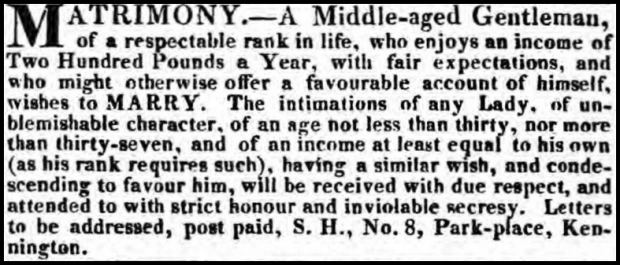
\includegraphics[width=0.45\textwidth]{figures/Introduction/morning-post-december-19-1822.png}\label{fig:img1_b}} 
    \caption{Matrimonial Advertisements in London’s \textit{Morning Post} in the 19th Century}
    \label{fig:img1}
\end{figure}

As the 19th century progressed, the popularity of matrimonial advertisements continued to grow, leading to the emergence of matrimonial specialty magazines like the Matrimonial News and the Matrimonial Intelligencer. These publications were dedicated solely to marriage and complemented the abundance of matrimonial ads found in newspapers, including those targeting specific religious audiences. Religion often played a significant role in these advertisements, highlighting the importance of shared faith in potential matches. Matrimonial ads provided an economical and accessible way for individuals who lacked family, friends, or financial resources to make meaningful connections and seek spouses.\cite{noauthor_alternative_2016}. Figure \ref{fig:img1} shows some of the examples advertisements posted in the newspapers during the 19th century. 

The concept of dating began to take shape at the turn of the 20th century, moving away from the more formal and structured courtship practices of earlier times. Dating became more informal and less focused on immediate marriage, reflecting broader social changes and evolving attitudes toward romantic relationships. This period saw the emergence of "dating" as a distinct phase of a relationship, where couples would spend time together outside the home without the immediate expectation of marriage. This shift was part of a larger cultural change that placed greater emphasis on personal choice and romantic love over social and economic considerations in mate selection. \cite{markarian_how_2017}. In the early 20th century, "Mechanical Matchmaking" emerged, with a notable example being the attempt by Hugo Gernsback, the publisher of Science and Invention magazine, to apply scientific methods to matchmaking. In April 1924, Gernsback proposed four "scientific" tests to determine the likelihood of marital success, including physical attraction tests, sympathy tests, body odor tests, and nervous disorder tests. These methods aimed to quantify and predict the success of marriages, illustrating an early fascination with applying technology and science to personal relationships, much like today's online dating algorithms.\cite{magazine_mechanical_nodate}. In the 1950s, a Newark based, matchmaking service called Introduction, used data as a foundation of their matchmaking services and charged a fee for ‘personalized’ recommendations of suitable matches based on qualifications and social status and subsequent sharing of contact information. \cite{newark_introduction_nodate}

One landmark development in the fusion of technology and dating was Operation Match, which emerged from Harvard University in 1965. Developed by undergraduate students Jeff Tarr and Vaughan Morrill, along with Doug Ginsberg and David Crump, Operation Match was conceived as an innovative solution to the challenges of dating life on campus. Utilizing an IBM 1401 computer, the service employed a sophisticated algorithm to match individuals based on their responses to a comprehensive questionnaire covering personal preferences and interests.\cite{noauthor_operation_1965}  Participants of Operation Match filled out lengthy questionnaires, which they submitted with \$3, and a program on an IBM 1401 computer would match questionnaires to similar responses.\cite{valley_new_2015}  The questionnaires were then transferred to punched cards and processed on an IBM 7090 computer and users received an IBM 1401 print out in the mail a week later, listing the names and contact information of potentially suitable matches. The increased sophistication provided by the IBM 1400 series propelled computer matchmaking into the public shhere as commercial matchmaking servics adopted advanced means to help singles find suitable dates. This increase in popularity of preferenced based match making combined with sexual revolution of the 1960s and 1970s, because of the introduction of oral contraceptives in the 1960s, the rising visibility of the LGBTQ+ community along with the second-wave of feminist movement,\cite{book:1309549} brought upon a drastic change in the attitudes of the people towards dating and relationships. From a culture that only endorsed serious relationships and marriage with the flexibility to choose a sociall equivalent partner, the society started to accept casual dating and hookups. The culture encouraged an individual to explore for their options both sexually and romantically, with multiple partners without any restrictions based on social strata and also having no end goal of marriage. The emergence of modern dating practices offered unprecedented opportunities for social mobility and the exploration of sexuality, albeit within the constraints of the era. This development represented a significant departure from traditional expectations, which often confined individuals to relationships with partners from specific, socially sanctioned groups. Women, in particular, experienced a notable expansion of autonomy through the relaxation of socio-cultural restrictions\cite{book:1309549}. This newfound freedom enabled them to date, form romantic attachments, and partake in sexual relationships with greater agency. 

\begin{figure}[t!]
 \centering
 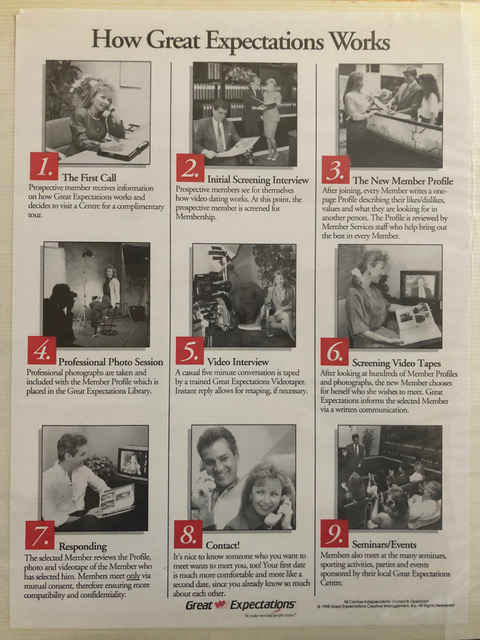
\includegraphics[scale=0.6]{figures/Introduction/GE2.png}
 \caption{A flyer explaining how Great Expectations works}
 \label{fig:img2}
\end{figure}

In the 1980s, post the rise of computer matchmaking, video matchmaking started to emerge. Video (or VHS) dating brought along with it a new way to meet potential partners, with added dimension of being able to hear and see the person before meeting them in person. The first known video dating service was started by Jeffrey Ullman in 1983, called the Great Expectations.\cite{waters_how_2021}. In video matchmaking, participants were asked a series of personal and motivational questions, such as their work ethic, triggers for anger, sources of motivation, and qualities they sought in a partner. After these interviews were recorded, the videotapes were cataloged in a video dating library. Members could browse through this collection, aided by a one-page profile attached to each video that included key details like height, location, and occupation, allowing them to screen potential matches before watching a tape. Figure \ref{fig:img2}, shows a flyer explaining how Great Expectations works. Hearing and Viewing the partners before selecting them was a significant advantage, because as Ullman said ``it showcased a more honest version of a person". \cite{waters_how_2021} This method brought out some of the marvellous personalities of people that would not show up just based on a written questionnaire as was the case in the previous approaches. But the hype of video dating dwindled in the early 1990s because of how cumbersome the process was. It did not bring out a massive change in the dating culture, but it did pave the way for the design of modern dating applications. 

The terminology "matchmaking" is purposefully employed in the preceding sections to delineate pre-Match.com "dating" mechanisms, as these early technologies primarily served the function of facilitating introductions between two parties deemed compatible on a multitude of criteria, ranging from social status to individual predilections and shared ideologies. Prior to the digital revolution instigated by Match.com, "dating" technologies were constrained to the matchmaking domain, enabling initial introductions without encompassing the subsequent phase of dating, which is crucial for assessing compatibility through real-world interactions. The advent of the internet, and specifically Match.com, heralded a paradigm shift by amalgamating matchmaking and dating within a unified online platform. Match.com was instrumental in revolutionizing the dating industry by accelerating the matchmaking process and introducing communication features like chat boxes, thereby allowing matches to engage in preliminary interactions ('date') prior to arranging face-to-face encounters.\cite{noauthor_dating_nodate} This platform introduced the concept of a 'dating profile', encouraging users to provide personal insights alongside photographs, thereby streamlining the process of discovering and interacting with potential matches within a singular service. Contrasting with prior methodologies, which necessitated intermediary involvement and were characterized by significant delays, online dating platforms provided immediate access to an expansive pool of potential matches, along with the autonomy to evaluate compatibility through direct communication, thus enhancing the process's transparency, dynamism, and efficiency.

The evolution of dating technologies further advanced with the development of mobile dating applications, such as Tinder and Bumble, transforming the dating experience into a mobile-centric endeavor. These applications, extensively discussed in the second chapter, innovated user interaction through the implementation of the 'swipe' mechanism and a pronounced focus on visual self-presentation\cite{noauthor_dating_nodate, marcus2016swipe} Notably, such applications significantly contributed to normalizing the sexual exploration or 'hook-up' culture, making it openly accessible and socially acceptable across various demographics\cite{noauthor_dating_nodate, marcus2016swipe}. Tinder, for instance, played a pivotal role in normalizing explicit expressions of sexual intentions by incorporating features that allow users to specify their looking-for preferences, such as casual encounters or long-term relationships, directly on their profiles. Employing sophisticated algorithms and engaging chat functionalities, including emojis, GIFs, and memes, these applications further refined the match screening process, enabling users to make more informed decisions regarding the viability of face-to-face meetings.

This transition from traditional matchmaking services to comprehensive online dating platforms has significantly broadened the interaction spectrum, empowering users to exercise greater selectivity in their dating pursuits. By facilitating a virtual screening process, these digital mediums have not only conserved time and effort but have also expanded the horizons for establishing and nurturing romantic connections in the contemporary era, underscoring a profound shift in the landscape of dating technologies.


\subsection{The Indian Context}
The evolution of dating and matrimony technologies in India has been influenced by the country's unique socio-cultural landscape, characterized by a rich tapestry of traditions, values, and familial structures. It is evident from the previous section that the Western dating culture has undergone significant transformations over the centuries, transitioning from arranged marriages to companionate marriages and subsequently embracing casual dating and hook-up culture. In contrast, to the technologies in the west, dating technology were modified to server as matrimonial services because of the social unacceptability of any form of Dating in the Indian society, until the 2000s \cite{doshi_date_2016, noauthor_modern_2017, sharma_towards_2019}. 

Traditionally, relationships and marriages in India were orchestrated through family networks or arranged by parents, emphasizing communal ties over individual choice. However, the late 20th and early 21st centuries marked a significant transition, driven by technological advancements and a growing emphasis on individual autonomy in choosing romantic partners. Personal advertisements were predominantly utilized to identify appropriate marital alliances, and the inception of Shaadi.com, shortly after the launch of Match.com, mirrored this utility, albeit within the matrimonial context of Indian society. In this cultural milieu, the responsibility of selecting suitable marital candidates traditionally rested with the parents, given the substantial emphasis placed on variables such as caste, religious affiliation, and upbringing. These factors not only held, but continue to hold, considerable importance, with parents extensively relying on their expansive social networks to discover apt matches for their offspring \cite{sharma_towards_2019, seth_online_2008}. Matrimonial services remained largely unchanged, focusing predominantly on matchmaking, as the prerogative to sift through recommended matches was vested in the parents of the concerned individuals, thereby obviating the necessity for incorporating 'dating experiences' to vet multiple prospective partners \cite{titzmann_changing_2013}. The paramount decision-making authority resided with the parents, thus constraining opportunities for dating or romantic exploration—until the widespread adoption of mobile phones in the early 2000s. Mobile telephony and the internet introduced novel avenues for discreet dating, facilitating the quest for partners beyond the traditional constraints of caste and religious affiliations. It is pertinent to highlight that, at this juncture, the Indian dating paradigm mirrored Western practices of the early twentieth century, predominantly aimed at culminating in 'love marriages.'

Liberalization of the Indian economy also played a pivotal role in the introduction of dating applications in India. Liberalization brought upon a transformation in the image of the traditional image of the middle-calss wife India. Traditionally, the middle-class wife in India was emblematic of virtues such as modesty, submissiveness, and a strong adherence to family values, often confined within the domestic sphere and her roles as a caregiver and moral guardian of the family. This portrayal underscored the gender norms and cultural expectations deeply ingrained in the patriarchal fabric of Indian society, where a woman's identity was largely defined through her relationships with men as a daughter, wife, and mother \cite{Dell_2005}.

The onset of economic liberalization introduced a wave of change, marking a pivotal shift in the socio-economic landscape of India. This period was characterized by the opening up of the Indian economy to global markets, an influx of foreign investment, and the adoption of neoliberal policies. Concurrently, this economic shift brought about a significant social transformation, particularly in the roles and perceptions of women in Indian society. The liberalization era ushered in increased educational and employment opportunities for women, challenging the traditional confines of their roles within the household and promoting a narrative of economic empowerment and independence for women. This marked departure from traditional roles was not merely an economic transition but also a cultural shift, fostering a reevaluation of gender dynamics and the emergence of new models of femininity and partnership inspired by global media and the internet \cite{Forbes_2020}.

The increased visibility of women in the workforce and their active participation in public and political spheres echoed the growing feminist movements in India. These movements advocated for gender equality, challenging the patriarchal status quo and pushing for legal and social reforms to address gender discrimination, marital rights, and issues of domestic violence. The discourse around marriage and relationships also evolved, reflecting a gradual shift towards mutual respect, companionship, and shared responsibilities between partners. The liberalization era, therefore, not only transformed the economic landscape but also significantly impacted the social fabric of India, reshaping traditional notions of womanhood and partnership \cite{statista_internet_users_2050}.

In the realm of dating and relationships, the impact of liberalization was further evidenced by the growing acceptance of love marriages, inter-caste and inter-religious unions, and the concept of dating itself—practices once considered taboo. 

The landscape of Indian dating culture witnessed a profound transformation in 2011 with Tinder's entry into the Indian market. Marketed primarily as a 'hook-up' application, Tinder swiftly gained traction among the youth, thereby democratizing dating and, notably, casual romantic encounters. The prevailing narratives suggest a gradual shift from a staunchly arranged marriage-oriented society towards a more open acceptance of 'dating' among the younger demographic. This cultural evolution is fostering the emergence of varied dating practices, spanning from serious relationships to casual dating and hook-ups. The locus of choosing a partner is increasingly transitioning from parents to the individuals themselves, buoyed by the rising popularity of online dating platforms such as OkCupid and Tinder. This paradigm shift towards individual agency in partner selection is a relatively recent development, with online dating gaining the quickest acceptance among college students and young professionals \cite{doshi_date_2016}.

The introduction of dating applications such as Tinder, OkCupid, and Bumble marked a significant cultural shift, offering an alternative to the traditional pathways to marriage. These platforms provided a space for individuals to explore romantic relationships without the immediate objective of marriage, thereby allowing for greater personal autonomy in matters of love and partnership \cite{Das_2019}. his shift is reflective of a broader global trend where individual choice and compatibility are increasingly valued over traditional matchmaking criteria.

The Chief Marketing Officer of OkCupid highlighted the unique nature of the Indian market, noting that a generation of young Indian women is redefining relationship norms by asserting their right to choose their partners. This sentiment encapsulates the transformative impact of dating apps, empowering individuals, especially women, to exercise greater control over their romantic lives "What makes India different is that we have a generation of young women who are changing things by saying, ‘I want to decide who I’m with’" \cite{Forbes_2020}.

In response to the cultural and societal nuances of the Indian context, homegrown applications like TrulyMadly and Aisle have emerged, blending traditional values with modern dating practices. These platforms are designed to cater to the Indian audience's preferences, striking a balance between casual dating and the pursuit of long-term partnerships. By incorporating cultural sensibilities into their algorithms and features, these apps offer a "middle ground" that respects the societal norms and expectations prevalent in Indian society \cite{Forbes_2020}. Bumble, in particular, has made a notable impact by emphasizing women's empowerment through its unique feature that allows only women to initiate conversations.\cite{noauthor_bumble_nodate} This approach not only challenges traditional gender dynamics but also promotes a safer and more respectful online dating environment for women, aligning with broader movements for gender equality and women's rights in India. The rise of dating applications in India is emblematic of the country's ongoing negotiation between tradition and modernity. As India continues to evolve socially and economically, these platforms reflect and facilitate changing attitudes towards relationships, marriage, and personal autonomy. Moreover, the success and adaptation of these platforms in India underscore the globalized nature of technological and cultural exchange, where Western innovations are localized to fit the specific needs and contexts of different societies.

The embrace of Bumble's features by women in India marks a notable shift in the country's dating culture. Women making the first move over 15 million times and sending twice the number of messages compared to the global average highlights a significant change in gender dynamics within the dating scene. This statistic not only signifies women's acceptance of the platform but also their active engagement in shaping their romantic interactions, which is a departure from the traditionally passive role attributed to women in the courtship process in India (Hindustan Times, 2020).

Moreover, the fact that 32\% of women users in India use more than one mode on Bumble suggests that the app is being used not just for dating but also for forming broader social connections. This indicates a broader application of the app's features, possibly extending to networking and friendship, reflecting a versatile use of technology to fulfill various social needs \cite{HindustanTimes_2020}. Further emphasizing the influence of contemporary culture on dating preferences, a recent Bumble report highlights how social media, music, food, literature, and content consumption are shaping Gen Z's dating ideals in India. These factors are indicative of a more globalized approach to dating where personal interests and cultural consumption significantly influence romantic connections \cite{Chronicle_2023}.

Additionally, changes in dating preferences show a trend towards virtual dating, with predictions that 40\% of single Indians will favor this mode of interaction. This reflects a growing comfort with digital interactions and an appreciation for the importance of education, career choices, and compatibility as bases for forming relationships, beyond just physical or geographical proximity \cite{MediaInfoline_2021}. The integration of technology into personal relationships is not unique to India. Globally, dating apps have reshaped social interactions. For instance, in the United States, Tinder and similar apps have significantly influenced dating norms, with studies indicating that online interactions have become a primary way young people connect romantically and socially. These platforms provide a space where users can express themselves in ways that may not be possible in their immediate physical environments, thus expanding their social horizons \cite{Smith_2016}.

The introduction of Bumble in India has marked a significant development in the visibility and social acceptance of LGBTQIA+ identities within the country. The platform’s proactive stance on inclusivity and safety has played a crucial role in not just providing a dating service but also advocating for the rights and recognition of LGBTQIA+ individuals in a society where their acceptance remains inconsistent. The decriminalization of gay sex by the Supreme Court of India in 2018 \cite{Johar} was a landmark moment, legally abolishing Section 377, a colonial-era law that criminalized homosexual acts. However, legal acceptance does not automatically translate into social acceptance, and the LGBTQIA+ community continues to face various forms of discrimination and stigma. In this context, platforms like Bumble serve as important spaces for safe social interaction and self-expression for LGBTQIA+ individuals.

Bumble has introduced several features aimed specifically at enhancing the safety and inclusivity of its platform for LGBTQIA+ users:

\begin{itemize}
    \item \textbf{Guides for Queer Dating:} Bumble provides tailored guides that offer advice and support for queer dating, addressing the unique challenges faced by LGBTQIA+ individuals in navigating the dating world. \cite{Bumble}
    \item \textbf{Incognito Mode:} This feature allows users to maintain privacy and control over who sees their profile, giving LGBTQIA+ users the discretion they may need in a conservative society. \cite{Bumble_incognito}
    \item \textbf{Private Detector:} Bumble’s private detector automatically blurs lewd images to protect users from unsolicited explicit images, enhancing the safety of interactions. \cite{Bumble_private_detector}a
    \item \textbf{Photo Verification:} This feature helps to ensure that profiles are genuine, reducing the risk of catfishing and improving trust and safety on the platform. \cite{Bumble_photo_verification}
    \item \textbf{Pronoun Selection:} By allowing users to select and display their pronouns, Bumble fosters an environment of respect and recognition for gender identity, which is particularly important for transgender and non-binary individuals. \cite{Bumble_pronoun_feature}
\end{itemize}

Bumble’s efforts extend beyond individual safety to influence broader social perceptions and norms regarding LGBTQIA+ identities. By normalizing the inclusion of diverse sexual orientations and gender identities in its platform, Bumble challenges societal prejudices and promotes greater visibility and acceptance of the LGBTQIA+ community. This visibility is crucial in changing public attitudes and encouraging more open discussions about LGBTQIA+ issues in India. Research on the impact of dating apps on LGBTQIA+ communities indicates that such platforms can significantly affect users' lives by providing spaces for identity exploration and community building that are often unavailable in other areas of their lives. Studies suggest that dating apps can help lower barriers to social interaction and empower users by allowing them to seek out connections on their own terms \cite{Blackwell_2015}. Moreover, the role of technology in shaping cultural and social dynamics is increasingly recognized, with scholars arguing that digital platforms can play a transformative role in challenging traditional norms and advocating for marginalized communities \cite{Publishers_Distributors4753/23_Road_Delhi}.

\section{Fairness in AI systems}
The widespread adoption of recommendation algorithms across digital platforms, ranging from online shopping to social media, has sparked a growing awareness of their capacity to perpetuate social injustices. These algorithms are fundamental in shaping user experiences by predicting and influencing behavior through the processing of vast datasets. However, despite their utility, they frequently mirror and even magnify existing societal biases, embedded unintentionally within the data they analyze. This issue arises from algorithms learning from real-world data that reflects historical inequalities or prevalent stereotypes, leading to decisions that systematically disadvantage certain groups.

The inadvertent reinforcement of biases by algorithms not only affects the fairness of automated decisions but also raises ethical concerns about the integrity of AI systems in various applications. As these systems become more integral to everyday life, the urgency for addressing these biases grows, necessitating a careful examination of how algorithms interact with societal norms and structures. Researchers have argued for the development of methods to detect and mitigate biases in AI systems as a critical step towards ensuring they promote equity and fairness. The challenge lies in the inherent complexity of AI models and the subtlety with which biases can be integrated into algorithmic decisions, often masked by the technical opacity of these systems.

Significant scholarly attention has been directed towards understanding the scope and impact of algorithmic bias. Studies have consistently highlighted the need for transparency in AI processes and the implementation of robust fairness metrics to evaluate and rectify biases. The push towards ethical AI involves a multidisciplinary approach, incorporating insights from computer science, social sciences, and legal studies to create AI systems that are not only effective but also equitable and just.

Therefore, addressing these challenges is not merely a technical task but a societal imperative, requiring concerted efforts from developers, regulators, and users alike. Ensuring the fairness of AI systems is fundamental to harnessing the full potential of this technology in a way that benefits all sections of society equitably, fostering trust and wider acceptance of AI applications across various domains.

In recent years, numerous cases have highlighted the inherent risks of discrimination and biases embedded in AI systems, particularly those used in recommendation engines and automated decision-making. These issues not only raise ethical concerns but also underscore the need for more robust frameworks to ensure fairness in AI deployments.

\subsection{Bias in Judicial Algorithms}
One of the most notable instances of AI bias is seen in the COMPAS algorithm, used in the criminal justice system in the United States. This algorithm was found to misclassify black defendants as having a higher risk of reoffending compared to their white counterparts, leading to unfairly harsher sentencing and bail decisions. This case underscored the racial biases that can be perpetuated by automated systems, raising alarms about the fairness and impartiality of using AI in legal contexts \cite{Mattu_COMPAS}.

\subsection{Bias in Job Advertisements and Recruitments}
Another significant example is the gender bias in job advertising on platforms like Facebook, where algorithms were found to display ads for high-paying job opportunities more frequently to men than to women. This was not the result of explicit programmer intent but rather the outcome of the algorithm learning from existing societal biases, indicating that without careful oversight, AI systems can reinforce and perpetuate existing inequalities \cite{Lambrecht_Tucker_2019}.

XING, a professional networking and job recruitment platform similar to LinkedIn, has also faced scrutiny for biases in its job recommendation algorithms. A notable instance of this was highlighted in a study that found XING's algorithms recommended more underqualified men for certain jobs than qualified women. This disparity suggests the presence of gender bias within the algorithm's decision-making processes. The study indicated that such biases could stem from the training data used to develop these algorithms. If the historical data on which these systems are trained contain gender imbalances—for instance, more men being hired for certain types of jobs than women—algorithms may inadvertently learn to perpetuate these patterns. This results in a feedback loop where men continue to be favored over equally or more qualified women, reinforcing gender inequality in professional settings.\cite{Lahoti_Gummadi_Weikum_2019}

In 2018, Amazon discovered that its AI-based recruitment tool exhibited bias against women. The AI was trained on resumes submitted to the company over a 10-year period, most of which came from men, reflecting male dominance in the tech industry. This historical data led the AI to favor male candidates over female candidates, penalizing resumes that included the word “women’s,” as in “women’s chess club captain.” Amazon eventually discontinued the use of the tool when it became clear that mitigating the bias was challenging. This case highlights the critical need to ensure diversity in training datasets and to continuously monitor AI systems for biases.\cite{Dastin_2018}

Datta et al. \cite{datta_automated_2015} in their study explore how platforms' algorithms use personal data to target ads, which can inadvertently reinforce societal biases. In the context of job advertisements, this targeting mechanism often prefers certain demographics over others based on historical data, leading to discriminatory practices. For instance, high-paying job ads might be shown predominantly to male users due to an algorithmic inference that links higher qualifications or job titles with male profiles, derived from biased historical hiring data. This form of bias not only limits the exposure of these opportunities to females but also perpetuates gender stereotypes in certain professions.

\subsection{Bias in Mortgage Applications}
AI systems have also been implicated in biases affecting mortgage approval processes. Research has shown that automated algorithms used by financial institutions to determine eligibility for loans were less likely to approve loans for applicants from minority backgrounds compared to similar white applicants. This kind of financial bias has significant long-term impacts on wealth accumulation and equality in access to housing \cite{Bartlett_Morse_Stanton_Wallace_2022}

\subsection{Bias in Facial Recognition Technologies}
Facial recognition technologies, widely used in surveillance and security applications, have been criticized for their higher rates of misidentification among people of color, particularly black individuals, and women. This not only raises privacy concerns but also poses a risk of wrongful accusations in law enforcement and security settings. Studies have shown that these biases are due to the underrepresentation of these groups in the training datasets used to develop these technologies \cite{Buolamwini_Gebru_2018}

Klare et al. \cite{Klare_Burge_Klontz_Vorder_Bruegge_Jain_2012} in their study examine how demographic variables, particularly race and gender, impact the accuracy of facial recognition systems. It reveals that these systems exhibit differential performance based on demographic groups, with notably lower accuracy rates for women and people of color compared to white men. The study underscores the challenges inherent in the training datasets used for developing these technologies, which often do not have a balanced representation of diverse faces. This imbalance leads to systems that are less effective at correctly identifying individuals from underrepresented groups, raising significant concerns about bias and fairness in security and surveillance applications where facial recognition technology is employed. The paper calls for improvements in dataset diversity and algorithm design to mitigate these biases and enhance the accuracy and reliability of facial recognition technologies across all demographic groups.

\subsection{Ethical Concerns in Healthcare Algorithms}
In healthcare, algorithms designed to predict patient health outcomes and allocate healthcare resources have shown biases against certain demographic groups. For example, an algorithm widely used in U.S. hospitals was found to be biased against black patients in its predictions of healthcare needs, resulting in less healthcare resources being allocated to black patients compared to white patients with similar conditions. \cite{Obermeyer_Powers_Vogeli_Mullainathan_2019}

\subsection{Other examples of Biases}
The paper "Unequal Representation and Gender Stereotypes in Image Search Results for Occupations" delves into the persistent issue of gender biases in image search results for various occupations. It highlights how popular search engines often reproduce and reinforce traditional gender stereotypes by displaying images that disproportionately represent men in certain professional roles while relegating women to more stereotypically 'feminine' jobs. This study systematically analyzes the search results for a range of job titles, illustrating a significant skew in the depiction of genders that aligns with societal stereotypes rather than actual workforce demographics. The findings of the paper suggest that such biased representations can have a profound impact on the perception of gender roles in society. For example, when a search for high-paying, prestigious professions like "CEO" or "engineer" predominantly returns images of men, it subtly suggests that these roles are more suited to men than women. Conversely, searches for roles such as "nurse" or "secretary" might yield an overwhelming majority of images of women, reinforcing the stereotype of these being women's work. The paper argues that these skewed images contribute to shaping and perpetuating gender biases, influencing both the aspirations of young people and the hiring decisions of employers. The authors call for more responsible curation of image results by technology companies to promote a more equitable and realistic portrayal of gender in professional contexts. \cite{Kay_Matuszek_Munson_2015}

Google Translate has shown signs of gender bias, especially in translating gender-neutral languages into English. For instance, Turkish sentences that include a profession or role, such as “doctor” or “nurse,” without a gender-specific pronoun, were translated into English with gender stereotypes: doctors became “he” and nurses became “she.” Google has acknowledged these biases and has updated its service to offer both feminine and masculine translations for single-word translations to mitigate this issue. \cite{Machine_Translation_Gendered_Innovations}

\section{Study of Technology, Sociocultural Dynamics, and Social Justice in Online Communities}
The intersection of technology and sociocultural dynamics within human-computer interaction (HCI) and social computing has garnered significant attention, particularly concerning power disparities and social justice issues. As online platforms increasingly influence social interactions and community structures, researchers have focused on how these technologies can be designed to foster positive community engagement and address social injustices. This body of research integrates insights from multiple disciplines, including behavioral economics, computer science, and sociology, to develop commitment mechanisms, participation controls, and incentive structures that support effective and equitable online communities.

\subsection{Engaging Ethical and Reflexive Design Practices}
Dombrowski et al. delve into the concept of social justice-oriented interaction design, urging the incorporation of ethical frameworks into technological products to tackle inherent biases and promote equality. The study proposes design strategies that prioritize social impacts and the collective well-being of users, pushing for an ongoing evaluation of technology's effects on society, particularly on marginalized groups. Their work underscores the importance of designers taking an active role in addressing ethical concerns and mitigating harm through deliberate design choices. This approach is positioned as essential for developing technologies that genuinely support social justice \cite{Dombrowski_Harmon_Fox_2016}.

\subsection{Interdisciplinary Approaches to Online Community Building}
Hutson et al. explore the potential of interdisciplinary approaches in crafting online communities that are not only engaging but also equitable. By integrating principles from behavioral economics, computer science, and social psychology, the authors argue for designing platforms that naturally encourage user participation while balancing power dynamics. Their study highlights specific commitment mechanisms and control features that can help maintain a fair and active community, suggesting that successful online platforms can emerge from the careful consideration of varied human factors and ethical considerations. This research is vital for understanding how diverse academic insights can converge to enhance user experience and community sustainability \cite{Hutson_Taft_Barocas_Levy_2018}.

\subsection{Incorporating Behavioral Economics for Effective Incentive Structures}
Kraut and Resnick provide a comprehensive overview of how behavioral economics can inform the design of online communities. The authors discuss the application of economic theories to predict and influence user behavior, thereby fostering environments conducive to cooperation and positive interaction. They outline various social mechanisms, such as rewards and reputation systems, which can incentivize users to contribute constructively to the community. Their framework also addresses potential pitfalls in community design, such as free-riding and conflict, proposing solutions based on empirical research and economic models. This study is particularly insightful for developers seeking to create engaging and sustainable online platforms \cite{Kraut_Resnick_2012}.

\subsection{Algorithmic Fairness in Social Platforms}
Selbst et al. investigate the complexities of implementing fairness in algorithmic systems, particularly within sociotechnical systems where human and machine interactions are deeply intertwined. Their research critiques simplistic approaches to fairness and advocates for a nuanced understanding of how algorithms can perpetuate or disrupt social norms. The study provides a theoretical foundation for developing algorithms that are not only technically efficient but also socially aware, offering guidelines for creating systems that are more just and equitable. This work is crucial for policymakers and technologists aiming to harness the benefits of AI without exacerbating social inequalities \cite{Selbst_Boyd_Friedler_Venkatasubramanian_Vertesi_2019}.

\subsection{Gender and Racial Biase in Algorithmic Recommendations}
MacLeod and McArthur (2019) analyze how dating apps like Tinder and Bumble shape user perceptions of gender through their interfaces and algorithmic recommendations. Their research identifies specific design elements that may reinforce traditional gender roles and exclude non-binary users. By conducting an interface analysis, they reveal how seemingly neutral technologies can carry implicit biases that affect user interactions and identity representation. The findings suggest that more inclusive design practices are needed to accommodate the diversity of user identities and preferences. This study is instrumental for developers and designers who aim to create more inclusive digital environments \cite{MacLeod_McArthur_2019}.

\subsection{Designing for Diversity and Inclusivity}
Zytko et al. propose a human-AI interaction framework for enhancing user safety in social matching apps, focusing particularly on marginalized users. The research advocates for participatory design methods that actively involve users from diverse backgrounds in the design process, ensuring that the resulting products are sensitive to the needs and safety concerns of all community members. This approach is aimed at preventing harm and improving the overall experience for users, especially those from the LGBTQIA+ community, by tailoring features to reflect real-world complexities and user-specific concerns \cite{Zytko_Furlo_Aljasim_2021}.

\section{Analysis of Biases in Online Dating Applications: A Focus on Bumble}
Online dating applications have become a ubiquitous feature of the social landscape, dramatically transforming how individuals connect and form relationships. These platforms offer unprecedented convenience and reach, enabling users to interact with potential partners beyond their immediate social circles and geographical boundaries. Among these platforms, Bumble has distinguished itself with unique features aimed at enhancing user autonomy and safety. However, the integration of these innovative online dating solutions has not been without its challenges.

The proliferation of online dating applications like Bumble has surfaced a range of biases that affect how individuals perceive each other and interact within digital spaces. These biases, whether embedded in the algorithmic frameworks that underpin user interactions or manifest in the design and policy decisions of the platforms, have significant implications for the user experience. They can influence user behavior, reinforce social stereotypes, and even exacerbate gender, racial, and sexual orientation disparities. Therefore, understanding and addressing these biases is crucial for creating more equitable and inclusive social platforms.

In this detailed analysis, we will explore various dimensions of biases in online dating applications, focusing particularly on Bumble. This exploration is grounded in academic research and augmented by recent studies that investigate how these biases manifest and the potential measures to mitigate their impact. Through this comprehensive review, we aim to shed light on the nuanced challenges and opportunities presented by online dating technologies, specifically examining how they shape user interactions and societal perceptions in the age of digital relationships.

We will begin by reviewing established research on Bumble's design and algorithmic impacts, followed by insights from new academic studies that offer contemporary perspectives on addressing these ongoing issues. This analysis seeks to provide a holistic understanding of the complexities involved in designing and managing online dating platforms that are not only technically efficient but also socially responsible and inclusive.

\subsection{Heteronormativity in Bumble's Design}
Bivens examines the infrastructure and safety features of Bumble, highlighting a design focus that predominantly caters to heterosexual interactions. The analysis suggests that such design choices are not merely reflective but also reinforcing of broader heteronormative biases prevalent within the tech industry. This predisposition in design philosophy may marginalize LGBTQ+ users by not adequately addressing their needs or by embedding heterosexual norms into the user experience and interaction dynamics on the platform. The study argues for a more inclusive design approach that recognizes and integrates diverse sexual orientations and gender identities \cite{Bivens_Hoque_2018}.

\subsection{Algorithmic Impacts on Society and Mental Health}
Yang explores the profound impact of dating app algorithms on societal structures and individual mental health. It underscores how algorithms can perpetuate existing social discriminations and gender inequalities. By leveraging user data, these algorithms can amplify societal biases, influencing how individuals perceive themselves and others. The study calls for algorithmic transparency and the development of ethical guidelines to govern algorithmic design, ensuring they do not reinforce harmful stereotypes or social hierarchies \cite{Yang_2021}.

\subsection{User Interface and Identity Representation}
The analysis of MacLeod and McArthur critiques the user interface (UI) of Bumble, arguing that its design is more aligned with the functional needs of matching profiles quickly rather than accurately representing user identities. This focus may lead to superficial interactions and misunderstandings, as the platform does not allow users to express nuanced aspects of their identities fully. The study suggests that dating apps should prioritize representational accuracy and depth in user profiles to foster more meaningful connections \cite{MacLeod_McArthur_2019}.

\subsection{Behavioral Patterns on Tinder: Gender Differences in User Engagement}
Tyson et al. research into user behavior on Tinder, another prominent online dating application, to provide a comparative perspective with behaviors observed on Bumble. Tyson and colleagues conducted a comprehensive analysis of user engagement patterns, specifically looking at how men and women interact with the platform. Their findings reveal significant gender differences in the way users approach potential matches. Men tend to be less selective, often swiping right (indicating interest) more frequently than women, irrespective of the match's details. In contrast, women are more selective and maintain a more deliberate pace in their interactions, often taking longer intervals between sending messages to potential matches. This study highlights the underlying gender dynamics that influence user strategies and interactions on dating apps. The behaviors observed reflect broader societal expectations and norms related to gender roles within the context of romantic and social interactions. Understanding these patterns is crucial for designing more inclusive and effective dating platforms that can cater to the diverse needs and behaviors of all users \cite{Tyson_Perta_Haddadi_Seto_2016}.

\section{Investigating Non-Binary Experiences on Dating Platforms in India}
The digital dating landscape has primarily focused on binary gender dynamics, often overlooking the rich spectrum of gender identities that users may identify with. Our study ventures into this less charted territory by specifically examining the experiences of non-binary individuals using dating platforms in India. This focus not only fills a significant gap in the existing literature but also enriches our understanding of the complexities involved in digital dating environments.Traditional studies on dating apps have predominantly concentrated on male and female user interactions, largely ignoring non-binary perspectives. By shifting the focus to non-binary individuals, our study acknowledges and addresses the diversity within gender experiences and challenges the binary normativity that prevails in most dating app research. 

The methodology of our study diverges from typical approaches by employing qualitative and quantitative measures specifically tailored to capture the nuanced experiences of non-binary individuals. This includes in-depth interviews, user experience surveys, and interaction analysis, providing a comprehensive view of their challenges and preferences on dating platforms. By focusing on Indian youth, this study explores a demographic that is rapidly embracing digital dating solutions but whose unique cultural and social dynamics are not well-documented in the context of non-binary experiences. India's complex landscape of traditional norms juxtaposed with modern influences makes it a particularly interesting case study for examining how non-binary individuals navigate dating platforms. Insights gained from this research can inform the development of more inclusive technologies. Understanding how non-binary users interact with existing platforms could lead to significant improvements in design, ranging from gender identity options to matching algorithms that account for diverse gender preferences and identities. This, in turn, can help create safer and more welcoming digital spaces for users who do not conform to traditional gender binaries. Beyond technological improvements, the findings can influence policies related to digital spaces and dating apps, advocating for greater recognition and protection of non-binary users. Community feedback mechanisms and support features could be developed based on the study's outcomes, fostering a more engaged and supportive community within these platforms.

While our study sets a foundation for exploring non-binary experiences in online dating within the Indian context, it also anticipates certain challenges. These include societal stigma, recruitment of participants, and the sensitivity required in handling personal and potentially vulnerable disclosures. Moving forward, the research aims to expand its scope to include a wider array of non-binary identities and explore intersectional factors such as religion, race, and socioeconomic status, which could further affect user experiences on dating platforms. In conclusion, by pioneering research into the experiences of non-binary individuals on dating platforms in India, this study not only contributes valuable insights to the academic community but also paves the way for more inclusive and empathetic technology design. It challenges existing paradigms and encourages a broader reconsideration of how digital tools cater to diverse user bases.

